\chapter{CHƯƠNG 4: ENCODER VÀ ỨNG DỤNG TRONG ĐIỀU KHIỂN ĐỘNG CƠ}
    \section{Khái niệm encoder}
        Encoder là một bộ cảm biến chuyển động cơ học tạo ra tín hiệu analog hoặc tín hiệu kỹ thuật số (digital) đáp ứng với chuyển động. Encoder có khả năng biến đổi chuyển động (chuyển động tịnh tiến, chuyển động quay của trục, ...) thành tín hiệu đầu ra số hoặc xung. Các thông tin được encoder chuyển đổi trong động cơ bao gồm
        \begin{itemize}
            \item Tốc độ quay của động cơ.
            \item Vị trí: độ dịch chuyển của trục động cơ so với vị trí ban đầu.
            \item Hướng quay: Tùy thuộc vào từng loại encoder.
        \end{itemize}


        \section{Phân loại}
        Các bộ mã hóa encoder có thể được phân thành các loại
        \begin{itemize}
            \item Bộ mã hóa quay (Rotary Encoder): hay còn gọi là bộ mã hóa trục, thu thập dữ liệu và cung cấp phản hồi dựa trên chuyển động quay của 1 đối tượng. Các lĩnh vực có nhu cầu sử dụng rotary encoder phải kể đến phản hồi động cơ, cánh tay robot. Rotary encoder được phân loại thành 2 loại là bộ mã hóa gia tăng (incremetal encoder) và tuyệt đối (absolute encoder). Bộ mã hóa gia tăng cung cấp thông tin vị trí góc tương đối bằng cách tạo ra một loạt xung khi trục quay, trong khi bộ mã hóa tuyệt đối cung cấp giá trị vị trí duy nhất cho mỗi vị trí trục, đảm bảo các phép đo chính xác và có thể lặp lại. 
            \begin{figure}[H]
                \centering
                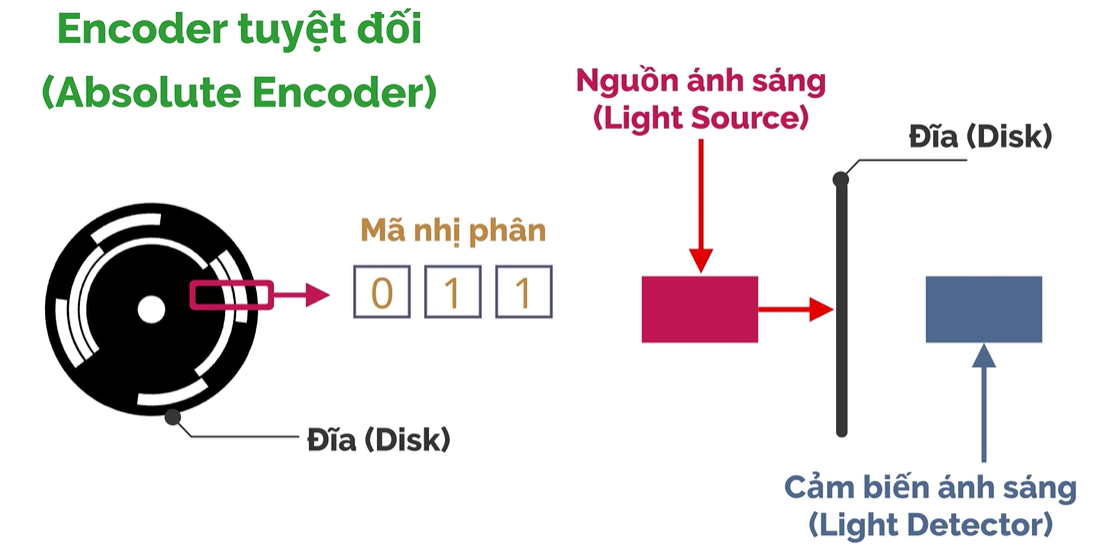
\includegraphics[width=1\textwidth]{pictures/encoder1.png}
            \end{figure}
            \begin{figure}[H]
                \centering
                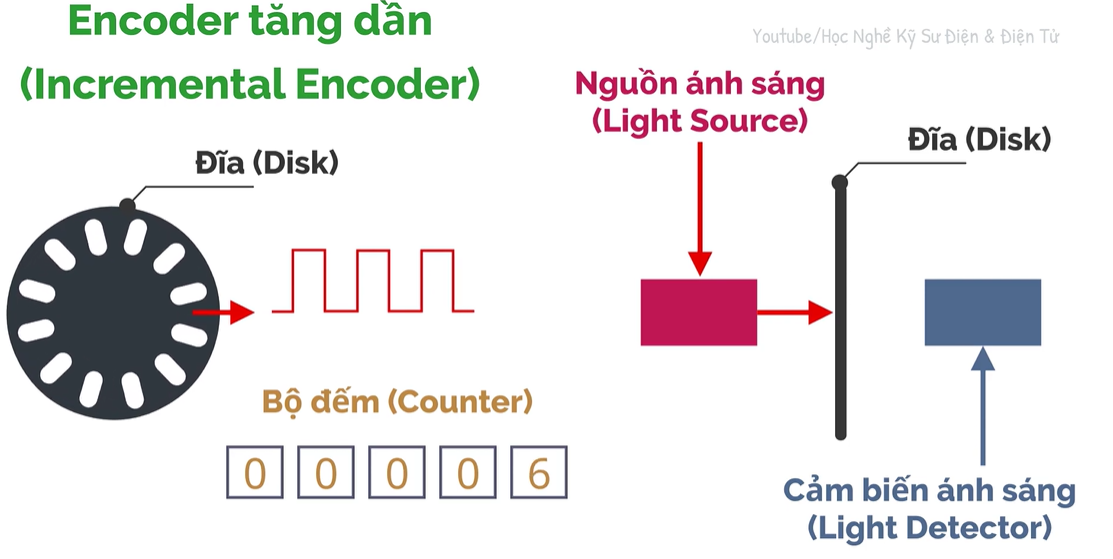
\includegraphics[width=1\textwidth]{pictures/encoder2.png}
            \end{figure}
            \item Bộ mã hóa tuyến tính (Linear encoders) được thiết kế để đo vị trí dọc theo đường thẳng, chúng thường được sử dụng trong máy CNC, dụng cụ đo chính xác và dây chuyền lắp ráp tự động. Encoder tuyến tính có thể là quang học hoặc từ tính. Bộ mã hóa quang học cung cấp độ phân giải và độ chính xác cao.
            \begin{figure}[H]
                \centering
                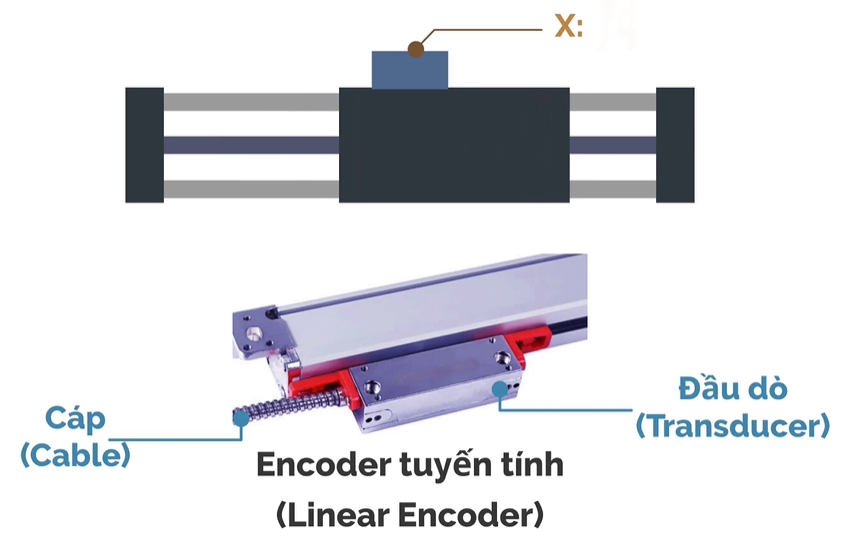
\includegraphics[width=0.7\linewidth]{pictures/encoder3.png}
            \end{figure}
        \end{itemize}
        Ngoài những phân loại chính, thì còn có phân loại theo những công nghệ dùng cho encoder, phổ biến là
        \begin{itemize}
            \item Quang học (Optical): Được sử dụng rộng rãi và phổ biến.
            \item Từ tính (Magnetic)
            \item Cơ học (Mechanical)
        \end{itemize}   
    \section{Cấu tạo của encoder}
        Mỗi loại bộ mã hóa (encoder) sẽ có thành phần chính và chức năng khác nhau, nhưng nhìn chung có 3 thành phần chính sau:
        \begin{itemize}
            \item Nguồn phát sáng (lightsource): là 1 đèn LED.
            \item Đĩa mã hóa (code disk): có rãnh nhỏ quay quanh trục, khi đĩa này quay và chiếu đèn LED lên trên mặt đĩa thì sẽ có sự ngắt quãng xảy ra. Các rãnh trên đĩa chia vòng tròn $360^{\circ}$ thành các góc bằng nhau. Một đĩa có thể có nhiều dãy rãnh tính từ tâm tròn.
            \item Bộ cảm biến ánh sáng thu tín hiệu (photosensor): là một con mắt thu quang điện để nhận tín hiệu từ đĩa quay
            \item  Bo mạch điện tử (electronic board): giúp khuếch đại tín hiệu
        \end{itemize}
        \begin{figure}[H]
                \centering
                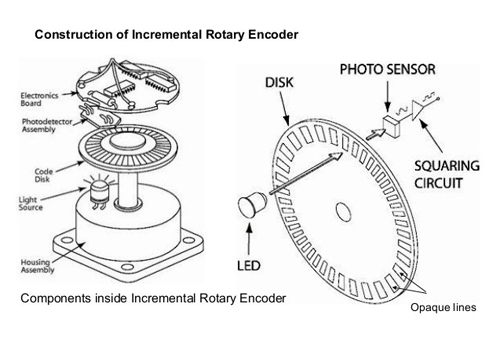
\includegraphics[width=1\linewidth]{pictures/encoder5.png}
            \end{figure}
        
        
        \cleardoublepage
        \subsection{Nguyên lý hoạt động của encoder}
        Encoder quay sử dụng quang học hoạt động theo nguyên lý đĩa quay quanh trục. Trên đĩa mã hóa có các rãnh nhỏ để nguồn phát sáng chiếu tín hiệu quang qua đĩa. Chỗ có rãnh thì ánh sáng xuyên qua được, chỗ không có rãnh ánh sáng không xuyên qua được.
        Với các tín hiệu có, hoặc không có ánh sáng chiếu qua, người ta ghi nhận được đèn led có chiếu qua lỗ hay không. Số xung đếm được và tăng lên được tính bằng số lần ánh sáng bị cắt.
        Cảm biến thu ánh sáng sẽ bật tắt liên tục để tạo ra các xung vuông. Việc sử dụng các bộ mã hóa sẽ ghi nhận lại số xung và tốc độ xung. Tín hiệu dạng xung sẽ được truyền về bộ xử lý trung tâm (vi xử lý, PLC,…) và từ đó kỹ sư cơ khí sẽ biết được vị trí và tốc độ của động cơ.
        \begin{figure}[H]
            \centering
            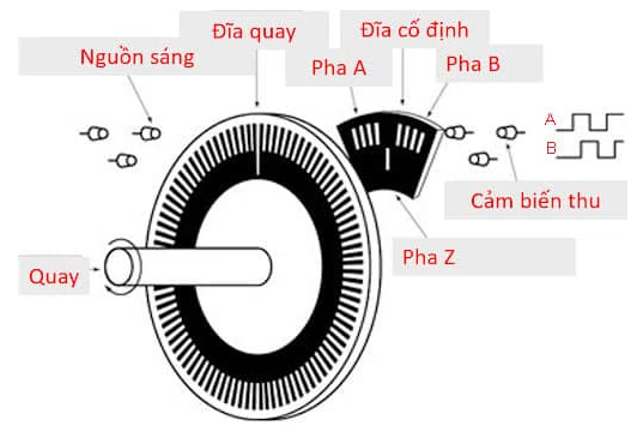
\includegraphics[width=0.8\linewidth]{pictures/encoder6.png}
        \end{figure}
        
        \cleardoublepage